\section{Evaluation}
\label{sec:eval}
We evaluated our system on the metrics of performance
and scalability. To measure performance, 
we designed benchmarks to measure the data rate 
of a listener versus the data rate of the host.
For scalability, we measured system 
performance as we added clients to the system. We can 
achieve this by launching our application on an 
increasing number of client machines.

\subsection{Performance}

For the performance of our system, we were interested in
differences in playback between clients in the same session.
We wanted clients to be listening to not just the same song,
but the same position in the song. To test this, we set up two
different experiments.

\begin{enumerate}

\item Determine differences in playback between a host and a
listener as more active sessions are added to the system.

\item Determine differences in playback between a host and a
listener as more listeners are added to their session.

\end{enumerate}

The host and listener were set up as different users on the same machine
so as to have identical clocks. The added sessions or listeners
were achieved through a modified version of Google's load test
for App Engine applications. Differences in playback were observed
through comparing the ending timestamps of songs between the host
and listener. Each experiment followed a similar series of steps,
listed below.

\begin{enumerate}

\item The host starts a session by choosing a song.

\item The listener joins the host's newly created session.

\item New sessions/listeners are added to the system.

\item The time the current song ended is recorded for both the
host and original listener.

\item The host adds a new song. Go to step 3.

\end{enumerate}

The results for adding more active sessions are shown in Figure
~\ref{fig:addSessions}. As more sessions were added to the system,
there wasn't much of a difference in song playback between the host
and listener. On average the difference actually decreased as more
sessions were added, but this is likely due to the outlier observed
for 30 sessions. The minor differences
observed are more likely to
have been caused by external network-related factors than by our
system itself.

\begin{figure}[h]
	\centering
	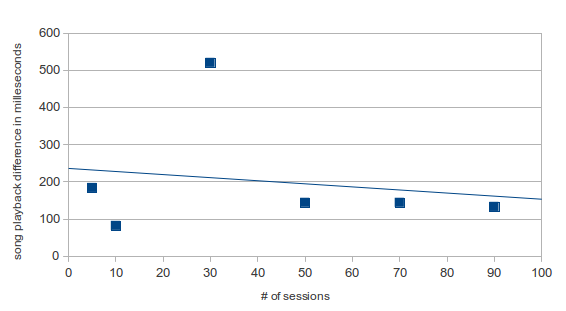
\includegraphics[width=0.5\textwidth]{add_sessions.png}
	\caption{Playback difference when adding more sessions.}
	\label{fig:addSessions}
\end{figure}

The results for adding more listeners are shown in Figure~\ref{fig:addListeners}.
As more listeners were added to a
session, there was a minor increase in song playback differences
between the host and listener. However, even with 90 active listeners
in a session, the difference was less than 1 second. This increase is
likely due to the additional work the server has to perform to
propagate updates to an increasing number of listeners in the
session.

\begin{figure}[h]
	\centering
	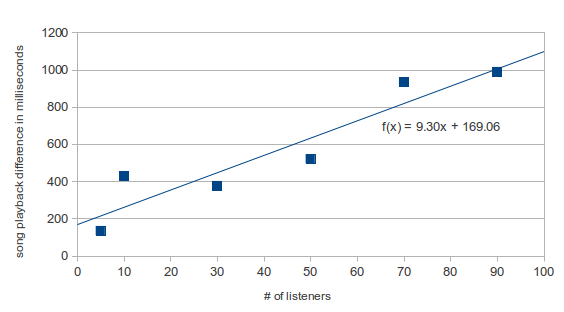
\includegraphics[width=0.5\textwidth]{add_listeners.png}
	\caption{Playback difference when adding more listeners.}
	\label{fig:addListeners}
\end{figure}

We also recorded the response time of our system as more listeners
were added to a session. The response time was calculated as the
elapsed time from the time of the client sent the request request
to the time the client
received a complete response from the server. The results are shown in
Figure~\ref{fig:addListenersResponseTime}. The response time
increased as more listeners were added to a session, starting at
around .5 seconds and reaching nearly 5 seconds. This is somewhat
expected as the server propagates session updates to all listeners
when a new listener joins a session. As more listeners join a
session, the server has to send more updates. Even with nearly
100 listeners, the response time was still under 5 seconds. This
is acceptable, but not ideal. To reduce this time, the server
could propagate updates only on song changes which would reduce
its overhead. However, this would cause hosts to have slightly
outdated session information.

\begin{figure}[h]
	\centering
	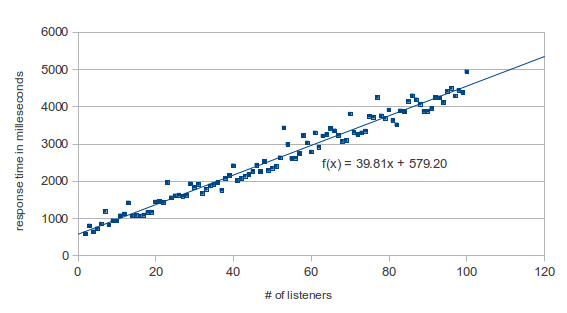
\includegraphics[width=0.5\textwidth]{add_listeners_response_time.png}
	\caption{Response time when adding more listeners.}
	\label{fig:addListenersResponseTime}
\end{figure}

\subsection{Scalability}
In terms of scalability, we tested how   
the number of listeners in a session 
would affect the amount of time it takes 
for a new user to join. 
To test this, we had one client start hosting a session and then had 
another user join the session as a listener. On joining, it would time 
how long it took to recieve a response from the data server. 
A minute later, another user would 
join the session to time how long it took the data server to respond to its request. 
We repeated this up to one hundred 
users. We stopped at one hundred  since we are limited to one hundred channels
and each user requires a channel. As you can see in Figure \ref{fig:addListenersJoinTime}, 
the first listener takes less than one second to join a music session 
whereas the the one hundredth user takes over four seconds to join a music session.  

\begin{figure}[h]
	\centering
	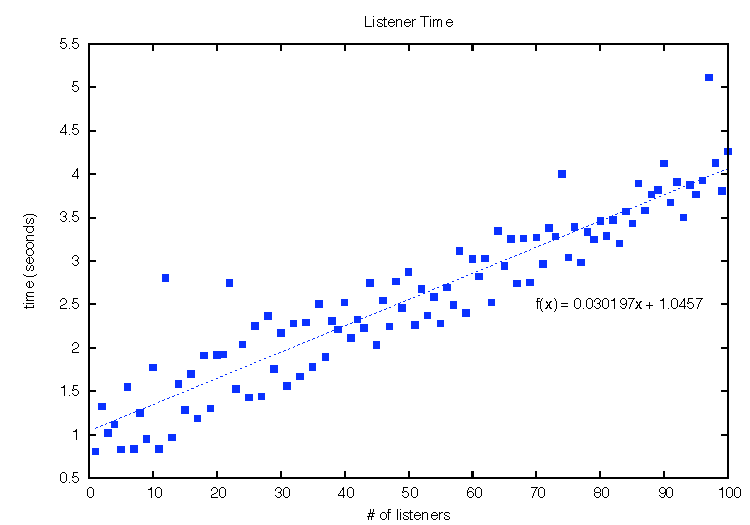
\includegraphics[width=0.5\textwidth]{deployed_time5.pdf}
	\caption{Time for listener to join a session}
	\label{fig:addListenersJoinTime}
\end{figure}
